%%%%%%%%%%%%%%%%%%%%%%%%%%%%%%%%%%%%%%%%%%%%%%%%%%%%%%%%%%%%%%%%%%%%%
%
% Author : Frederic Petrot
% Modified by : Olivier Sirol
% $Id: overview.tex,v 1.4 2000/04/17 12:02:03 czo Exp $
%
%%%%%%%%%%%%%%%%%%%%%%%%%%%%%%%%%%%%%%%%%%%%%%%%%%%%%%%%%%%%%%%%%%%%%
\documentclass{article}
\usepackage{t1enc,isolatin1}
\usepackage{palatino,psfig,here}
\textheight 9.0in
\textwidth 6.0in
\topmargin -0.0in
\oddsidemargin +0.3in
\evensidemargin -0.3in
\marginparwidth +0.5in
\parskip 8pt plus 2pt minus 2pt % space beetween paragraphe
\parindent 0em % indentation of the first line
\topsep 0pt % space beetween list and text
\parsep 8pt % space beetween 2 par.
\partopsep 0pt % space beetween 2 par.
\itemsep 0pt % space beetween 2 items
\raggedbottom
\begin{document}
%\psdraft
%%%%%%%%%%%%%%%%%%%%%%%%%%%%%%%%%%%%%%%%%
%
%
%%%%%%%%%%%%%%%%%%%%%%%%%%%%%%%%%%%%%%%%%%%%%%%%%%%%%%%%%%%%%%%%%%%%%
\begin{center}
\Large \textbf{Alliance}: A Complete CAD System for \textbf{VLSI} Design\\
\vspace*{1cm}
\large
�quipe Achitecture des Syst�mes et Micro-�lectronique\\
Laboratoire d'Informatique de Paris 6\\
Universit� Pierre et Marie Curie\\
4, Place Jussieu 75252 Paris Cedex 05,\\
France\\
\texttt{http://www-asim.lip6.fr/alliance/}\\*
\texttt{ftp://ftp-asim.lip6.fr/pub/alliance/}\\*
\texttt{mailto:alliance-support@asim.lip6.fr}\\*
\end{center}

%%%%%%%%%%%%%%%%%%%%%%%%
%
%%%%%%%%%%%%%%%%%%%%%%%%%%%%%%%%
\section*{\centerline{Abstract}}
\begin{quote}\em
The \textbf{Alliance} package is a complete set of CAD tools for the
specification, design and validation of digital \textbf{VLSI} circuits.
Beside the tools, \textbf{Alliance} includes also a set of cell 
libraries, from standard cells for automatic place and route tools, 
to custom block generators to be used in high performance circuits.
This package is used in more than 250 universities worldwide.

Each \textbf{Alliance} tool can operate as a standalone program as 
well as a part of the complete design framework.
After introducing briefly the design methodology, we outline the
functionnality of the tools.
Experiemental results conclude the presentation.

\textbf{Alliance} runs on any \textbf{Unix} system and has been recently
ported to \textbf{Windows} NT.
It is freely available on \texttt{ftp}, 
and includes binaries, leaf
cells libraries, on-line documentation, and tutorials.
\rm\end{quote}




%%%%%%%%%%%%%%%%%%%%%%%%%%%%
%
%%%%%%%%%%%%%%%%%%%%%
\section{Introduction}

The \textbf{Alliance} package is the result of a ten years effort 
spent at the \textbf{LIP6} Laboratory (formerly \textbf{MASI}) 
of the Pierre et Marie Curie University (UPMC), in Paris.
During these years, our major goal was to provide our undergraduate 
and graduate students with a complete CAD framework, designed to 
assist them in digital \textbf{VLSI} \textbf{CMOS} course.
The \textit{Architecture} team at \textbf{LIP6} focuses its activity on 
two key issues: computer architectures using high complexity ASICs, 
and innovative CAD tools for \textbf{VLSI} design.
Strong interaction exists between the people working on computer 
architectures and the one working on CAD tools.
The main CAD action aims at fulfilling both the needs of experienced 
designers by providing practical answers to state-of-the-art problems 
(logic synthesis, procedural generation, layout verification, test and
interoperability), and novice designers, by providing a simple and
consistent set of tools.
Our \textbf{VLSI} design flow is therefore based on both advanced CAD tools 
that are not available within commercial CAD systems, such as 
functional abstraction or static timing 
analysis, and standard design/validation tools.

\textbf{Alliance} VLSI CAD System is free software. Binaries, source code and 
cells libraries are freely available under the GNU General Public Licence (\textbf{GPL}).
You are welcome to use the software package even for commercial designs whithout 
any fee. You are just required to mention : "Designed with Alliance � LIP6/Universit� 
Pierre et Marie Curie". For any questions please mail to : 
\texttt{alliance-support@asim.lip6.fr}.



%%%%%%%%%%%%%%%%%%%%%
%
%%%%%%%%%%%%%%%%%%%%%%%%%%%%%%%%%%%%%%%%%%
\subsection{Process independence}

To be useful, a CAD system must provide a way to the silicon,
therefore \textbf{Alliance} provides a large set of cell libraries
also available at the layout level.
The target technologies of \textbf{Alliance} is \textbf{CMOS}.
The layout libraries rely on a symbolic layout approach that provides 
process independence in order to allow the designers to easily
port their designs from one silicon supplier to another.
The main point in this approach is that the pitch matching constraints
in both \textit{x} and \textit{y} direction are kept through
technological retargetting.
The translation, fully automated, relies on a technological file
suited to a given process.

These files can be generated directly from the process design rules.
Also technological files for several processes are available through
the CMP and EuroPractice services, provided you signed a NDA for the
process.

%%%%%%%%%%%%%%%%%%%%%
%
%%%%%%%%%%%%%%%%%%%%%%%%%%%%%%%%%%
\subsection{Software portability}

The \textbf{Alliance} package has been designed so to run on an
heterogeneous network of workstations.
The only requirements are a \textbf{C} compiler and a \textbf{Unix} system.
For the graphical applications, the XWindow library is used.
Several hardware platforms, from Intel 386 based microcomputers to
SparcStations and DEC Stations, are supported.

%%%%%%%%%%%%%%%%%%%%%
%
%%%%%%%%%%%%%%%%%%%%%%%%%%%%%%%%%%

\subsection{Modularity}

According to the interoperability constraints, each \textbf{Alliance} 
tool can operate as a standalone program as well as a part of the 
complete \textbf{Alliance} design framework.
Each \textbf{Alliance} tool therefore supports several standard \textbf{VLSI} 
description formats : \textbf{SPICE}, \textbf{EDIF}, \textbf{VHDL}, \textbf{CIF},
\textbf{GDS2}.
In that respect, the tools ouputs are fully usable under the
\textbf{Compass} and \textbf{Cadence Opus} environnement, provided these
tools have the necessary configuration files.
The \textbf{Alliance} tools support a zero-default top-down design
methodology with not only construction tools --- layout editor, automatic
place \& route --- but also validation tools, from design rule checker to
functional abstraction and formal proof.

%%%%%%%%%%%%%%%%%%%%%     
%                                                                    
%%%%%%%%%%%%%%%%%%%%%%%%%%%%%%%%%%                                   
\subsection{Compactness}

Unlike commercially available CAD systems, the \textbf{Alliance} CAD 
Framework suits the limited ressources of low-cost workstations.
For small educational projects --- 5000 gates ---, a \textbf{Unix} 
system with 8 to 20 Mbytes of memory, appropriate disk storage (30 
Mbytes per user), and graphic capabilities (X-Window) is sufficient.

%%%%%%%%%%%%%%%%%%%%%
%
%%%%%%%%%%%%%%%%%%%%%%%%%%%%%%%%%%
\subsection{Easiness}

All tools and the proposed design flow are simple to teach and to 
learn.
In any situation, easiness and simplicity have been prefered to 
sophisticated approaches.

To each tool correspond a unique behavior and utility.
Each step of the design methodology corresponds to the use of one or a
few tools, for which the usage is well identified.

From a pratical point of view, both on-line documentation (\textbf{Unix}
\texttt{man}) and paper are available with each tool of the
\textbf{Alliance} package.

%%%%%%%%%%%%%%%%%%%%%        
%        
%%%%%%%%%%%%%%%%%%%%%%%%%%%%%%%%%%        
\section{Alliance design flow}

We refer to the term "design flow" as a sequenced set of 
operations performed when realizing a \textbf{VLSI} circuit.
In the design flow, we rely on a strict definition of all the
objects and design functions found in the process of designing a
\textbf{VLSI} chip.
The design flow is based on the Mead-Conway model and is 
characterized by its top-down aspect.
Below we introduce the major steps of the basic design methodology.
It emphasizes the top-down aspect of the design flow, and points out 
that our methodology is breaked up into 5 distinct parts, the latter 
being not available yet within \textbf{Alliance}:
\begin{itemize}
\item capture and simulation of the behavioral view,
\item capture and validation of the structural view,
\item physical implementation of the design,
\item layout verification,
\item test and coverage evaluation.
\end{itemize}

The design flow also includes miscellaneous tools like layout editor
for the design of the cell libraries, and a PostScript plotter for
documentation.

%%%%%%%%%%%%%%%%%%%%%        
%        
%%%%%%%%%%%%%%%%%%%%%%%%%%%%%%%%%%        
\subsection{Capture and simulation of the behavioral view}

Like we just saw, the capture of the behavioral view is the
very first step of our design flow.
Within \textbf{Alliance}, any \textbf{VLSI} design begins with a timing 
independent description of the circuit with a subset of \textbf{VHDL} 
behavior primitives.
This subset of \textbf{VHDL}, called \texttt{vbe}, is fairly 
restricted: it is the data-flow subset of this language.
It is not very easy to modelize an architecture using this subset, 
but it has the great advantage of allowing simulation, logic synthesis
and bit level formal proof on the same files.

Patterns, \textbf{VHDL} simulation stimuli, are described in a specific 
formalism that can be captured using a dedicated language \texttt{genpat}.
Once a \textbf{VHDL} behavioral description written and a set of test vectors 
have been determined, a functional simulation is ran.
The behavioral \textbf{VHDL} simulator is called \texttt{asimut}.
It validates the input behavior, according to the input/output vectors.


%%%%%%%%%%%%%%%%%%%%%
%
%%%%%%%%%%%%%%%%%%%%%%%%%%%%%%%%%%
\subsection{Capture and validation of the structural view}

The structural view can be captured once the data flow description 
is validated.
The actual capture of the netlist relies either on specific 
description languages, \texttt{genlib} for standard cells or \texttt{fpgen}
for data-path, or on direct synthesis from the data flow  using the
\texttt{bop} tool for optimization and the \texttt{scmap} tool to map
on a cell library.
\texttt{Genlib} and \texttt{fpgen} are netlist-oriented libraries of C 
functions.
In the design methodology, it is essential for the students to get 
acquainted with the \textbf{C} language basics.
The advantage of such an approach is that designers do not have to 
learn several language with specific syntax and semantics.

Usually, the main behavior is partitionned in several sub-behaviors.
Some are described recursively using the \texttt{genlib} language, other
using \texttt{fpgen}, and the other ones can be directly synthesized 
from a \textbf{VHDL} description of the corresponding sub-behaviors.
The \texttt{scmap} tool takes an \textbf{RTL} description and 
generates a netlist of standard cell gates.
An other subset of \textbf{VHDL} allows to capture finite state machines.
This subset, called \texttt{fsm}, can be translated into a 
\textbf{RTL} description using the tool \texttt{syf}, and then the 
resulting description optimized usign \texttt{bop} and finally 
syntesized as a netlist using once more \texttt{scmap}.

Since \texttt{asimut} can operate on both \textbf{RTL} and structural views,
the structural description is checked against the behavioral 
description by using the same set of patterns that has been used for
behavioral validation.

%%%%%%%%%%%%%%%%%%%%%
%
%%%%%%%%%%%%%%%%%%%%%%%%%%%%%%%%%%
\subsection{Physical design}

Once the circuit netlist has been captured and validated, each leaf of
the hierarchy has to be physically implemented.
A netlist issued from \texttt{scmap} is usually placed and routed using
the standard cell router \texttt{scr}.
If the netlist has been captured using \texttt{genlib} and if it has a
high degree of regularity, it can be placed manually for optimisation
using other \texttt{genlib} functions.
The netlist resulting from the use of \texttt{fpgen} are placed and
routed using the datapath router \texttt{dpr}.

These part can be assembled together using a gridless channel router
called \texttt{bbr}, and this generates what we call a \textit{core}.
The circuit core is now ready to be connected to external pads.
The core-to-pads router, \texttt{ring}, aims at doing this operation 
automatically, provided the user has given an appropriate netlist and
some indications on pad placement.

The last stage of the physical implementation is the translation of
the symbolic layout to a foundry compliant layout using the 
\texttt{s2r} tool.
After that, the tape containing the circuit can be processed by the
silicon supplier.

%%%%%%%%%%%%%%%%%%%%%
%
%%%%%%%%%%%%%%%%%%%%%%%%%%%%%%%%%%
\subsection{Verification}

In our \textbf{VLSI} class, we intend to show that \textbf{VLSI} 
verification is at least as important as \textbf{VLSI} physical 
design.
For that reason, we have introduced in the design flow powerful tools 
to perform behavior, netlist and layout verifications.

The correctness of the design rules is checked using the design rule
checker \texttt{druc}.

An extracted netlist can be obtained from the resulting layout.
\texttt{Lynx}, the layout extractor operates on both hierarchical and 
flattened layout and can output both flattened netlists (transistor 
netlist) and hierarchical netlists.
The transistor netlist is the input of the \texttt{yagle} functional 
abstractor.
\texttt{Yagle} provides a \textbf{VHDL} data-flow behavioral 
description, identical to the one that feeds \texttt{asimut},  from 
the transistor netlist of a circuit.
The resulting behavior can be compared to the initial specifications
using either \texttt{asimut} with the functionnal vectors used for the
validation of the behavioral specification, or formally proved
equivalent, thanks to the formal proof analyzer \texttt{proof}.

When extracted hierarchically, the resulting netlist can be compared 
with the original netlist by using the \texttt{lvx} tool.
\texttt{Lvx}, that stands for Logical Versus Extracted, is a netlist 
comparator that matches every design object found in both netlists.

The critical path of the circuit, and an estimate of its delay, can be
obtained using the static timming analyzer \texttt{tas}.

%%%%%%%%%%%%%%%%%%%%%
%
%%%%%%%%%%%%%%%%%%%%%%%%%%%%%%%%%%
\subsection{Test and coverage evaluation}

For now, the fault coverage provided by the functional patterns is
evaluated using a commercial fault simulator, as \textbf{Alliance}
doesn't provide one yet.

%%%%%%%%%%%%%%%%%%%%%                            
%                            
%%%%%%%%%%%%%%%%%%%%%%%%%%%%%%%%%%                            
\section{Tools and layout libraries of the \textbf{Alliance} package}

Every \textbf{Alliance} tool has been designed to simply interface with 
each other, in order to support the proposed design flow.
Nevertheless, each tool can also be used independently, thanks to the 
multiple standard formats used for input and output files.

One of the most important characteristics of the \textbf{Alliance} system is 
that it provides a common internal data structure to represent the 
three basic views of a chip: 
\begin{itemize}
\item the behavioral view,
\item the structural view,
\item the physical view.
\end{itemize}

Figure~\ref{tools} details how all the \textbf{Alliance} tools are linked 
together around the basic behavioral, structural and physical 
data structures.

\begin{figure}\center
\leavevmode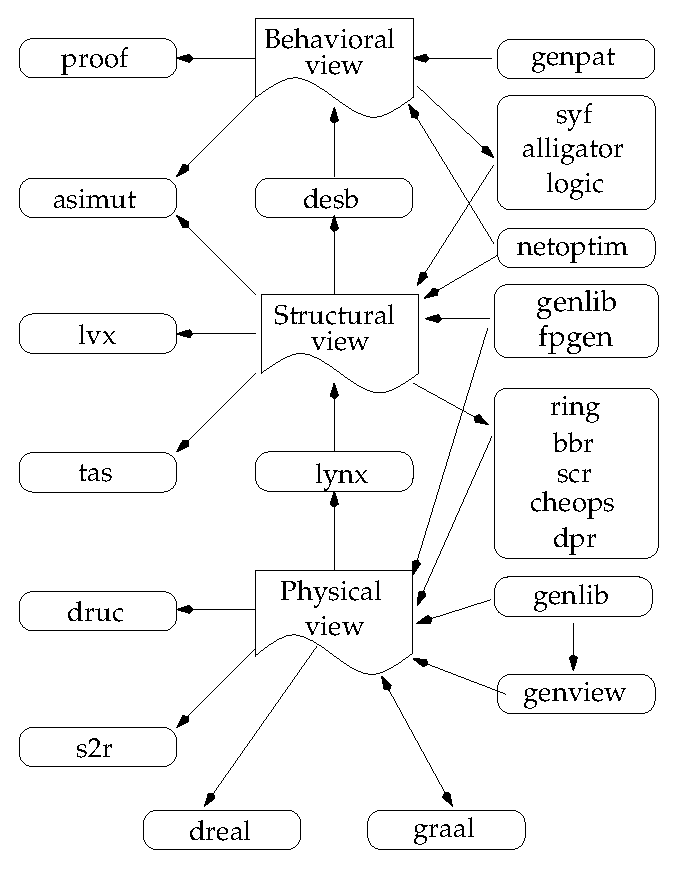
\psfig{file=tools.eps,width=8cm}
\caption{\label{tools}How the tools are linked on the data structures.}
\end{figure}

The process independence goal is achieved with a thin fixed-grid 
symbolic layout approach.
All the library of the system use this approach successfully.
Layouts have been targetted to ES2 2$\mu$m, 1.5$\mu$m, 1.2$\mu$m,
1.0$\mu$m and 0.7$\mu$m technologies, the AMS 1.2$\mu$m technology and
SGS-Thomson 0.5$\mu$m technology.
Chips have been fabricated successfully through the \textbf{CMP} services on
these technologies.

%%%%%%%%%%%%%%%%
%
%%%%%%%%%%%%%%%%%%%%%%%%%%%%%%%%%
\subsection{Tools}

\begin{itemize}
\item \texttt{asimut} is a \textbf{VHDL} logic simulator.
      The supported \textbf{VHDL} subset allows both structural and behavioral 
      data-flow description (without timing information).  
      Complex systems and microprocessors, including \textbf{INTEL} 8086 and 
      \textbf{MIPS} R3000 have been successfully simulated with \texttt{asimut}.
      \texttt{Asimut} is based on an event-driven algorithm and powerful 
      representation of boolean functions using binary decision
      diagrams.

\item \texttt{genpat} is a language interpreter dedicated to efficient 
      descriptions of simulation stimuli.
      It generates an \textbf{ASCII} file that can act as an input of 
      \texttt{asimut}.
      A \texttt{genpat} file format to \textbf{MSA} translator allows the 
      generation of appropriate simulation patterns for the Tektronix 
      LV500 tester.
      This allows to perform functional tests when the circuits comes
      back from the foundry.

\item \texttt{glop} is a gate level netlist optimizer.
      If the output of the logic synthesis takes into account the
      internal delays of the cells during the mapping phase, it 
      doesn't take into account the fan-out problems.
      \texttt{Netoptim} work is to ensure that the drive capabilities of
      all cells are correct, and to try to minimize the delays on the
      critical pathes in inserting buffers where appropriate.

\item \texttt{genlib} is a procedural language for netlist capture and 
      placement description (there is no schematic editor in the
      \textbf{Alliance} system).
      \texttt{Genlib} provides a consistent set of \textbf{C} 
      primitives, giving the designers the ability to describe 
      \textbf{VLSI} circuit netlists in terms of terminals, signals 
      and instances, or circuit topologies in terms of placement of 
      abutment boxes.  
      \texttt{Genlib} is mainly used to build parameterized netlist and
      layout generators.

\item \texttt{genview} is a debugging tool for the development of the
      layout view of parameterized generators.
      It is a graphical environment that integrates a \texttt{genlib}
      interpreter, a step by step debugger, and a window in the which 
      the circuit under construction is visualized.
      All the parameterized generators of \textbf{Alliance} have been
      developed using this tool.
      Part of the \textit{ROM} generator \texttt{grog} under construction
      is shown figure~\ref{genview}.
      
      \begin{figure}\center
%      ,angle=-90}
         \leavevmode\psfig{file=genview.eps,width=5cm}         
         \caption{\label{genview}A typical run of \texttt{genview}.}
      \end{figure}

      \texttt{Genview} uses the GNU \texttt{gcc} compiler parameterized for
      a virtual architecture as basis to its \texttt{genlib} interpreter.

\item \texttt{fpgen} is a language that has moreorless the same
      functionalities as \texttt{genlib}, but it is dedicated to datapath
      description.
      Its primary difference with \texttt{genlib} is that it allows to
      manipulate vectors of cells, like 32 two inputs \texttt{nand} gates
      or a 32 bits adder.
      It contains many primitives that greatly simplify the
      description of operative parts, in an optimized manner.

\item \texttt{bop} is a logic optimizer and logic synthesis tool.
      The input file is a behavioral description of the circuit using 
      the same \textbf{VHDL} subset as the logic simulator.
      The boolean equations described in \textbf{VHDL} are optimized so
      to minimize the number of boolean operators.
      The output is a new, optimized, data flow description.

\item \texttt{scmap} is a logic synthesis tool.
      The output is a netlist of gates.
      \texttt{scmap} can map a data-flow description on any 
      standard-cell library, as long as a \textbf{VHDL} data-flow
      description is provided with each cell.

\item \texttt{c4map} is a logic synthesis tool.
      It has the same functionnality than \texttt{scmap}, but runs 
      without a predefined standard-cell library, thanks to an 
      internal cell compiler.

\item \texttt{syf} is a finite state machine synthesizer.
      More precisely, \texttt{syf} assigns values to the symbolic states
      used for the automaton description, and aims at minimizing the
      resulting logic for both state transistion and output generation.
      The input is a \texttt{fsm} description, using a dedicated subset
      of \textbf{VHDL} that includes process description.
      The output is a behavioral description of the circuit using 
      the same \textbf{VHDL} subset as the logic simulator.
      The output of \texttt{syf} is to be synthesized into a netlsit of
      gates using \texttt{scmap}.

\item \texttt{scr} is a place and route tool for standard-cells.
      The placement system is based on simulated annealing.
      The channel router is an adaptation of the greedy router of
      Rivest-Fidducia.
      Feed-throughs and power routing wires are automatically 
      inserted where needed.
      The input is a netlist of gates.
      The output is either an hierarchical (channels are 
      instanciated) or flattened (channels are inserted) chip core 
      layout without external pads.  
      A specialized router is used for core to pad routing.
      
\item \texttt{Dpr} is a place and route tool for bit slice oriented 
      datapath.
      It privilegies the direct connexions between cells, and allows
      to used optimized blocks, like a fast multiplier or a register
      file, within the datapath.
      \begin{figure}\center
      \leavevmode\psfig{file=datapath.eps,width=5cm}
      \caption{\label{dpr} Part of a datapath.}
      \end{figure}
      Most parameterized generators available in \textbf{Alliance} follow
      the bit-slice structure of this datapath compiler.
      This tool allows to mix some glue logic directly within a
      datapath.
      This functionnality doesn't exist in commercial tools.

\item \texttt{bbr} is a gridless channel router that allows to route
      together two blocks having different topologies.
      For example the control part of a microprocessor realized in
      standard cell, and its operative part done as a datapath.
      \texttt{Bbr} is pretty tricky, and should be used with care.

\item \texttt{Ring} is a specific router dedicated to the final routing 
      of chip core and input/output pads.
      \texttt{Ring} takes into account the various problems of pad 
      placement optimization, power and ground distribution.
      A set of symbolic pads is included in the package.

\item \texttt{S2r} is the ultimate tool used in our design flow to 
      perform process mapping.
      \texttt{S2r} stands for "symbolic to real", and translates the 
      hierarchical symbolic layout description into physical layout 
      required by a given silicon supplier.
      The translation process involves complex operations such as 
      denotching, oversizing, gap-filling and layer adaptation.
      Output formats are either \textbf{CIF} or \textbf{GDSII}.
      \texttt{S2r} requires a parameter file for each technology aimed at.
      This file is shared with \texttt{druc}, \texttt{lynx}, \texttt{graal},
      \texttt{dreal} and \texttt{genview}.
      From an implementation point of view, these tools use a 
      bin-based data-structure that has very good performances.

\item \texttt{druc} is a design rule checker.
      The input file is a - possibly hierarchical - symbolic layout.
      It checks that a layout is correct regarding the set of symbolic
      design rules.
      This correctness must be ensured in order for \texttt{s2r} to
      produce a layout compatible with the target silicon foundry.

\item \texttt{Lynx} is a layout extractor.
      The input is a - possibly hierarchical - layout.
      The layout can be either symbolic or real.
      The output is an extracted netlist with parasitic capacitances.
      The resulting netlist can either be hierarchical or flattened 
      (transistor netlist).


\item \texttt{Lvx} is a logical versus extracted net-compare tool.
      The result of a run indicates if the two netlist match together,
      or if there are different.
      Note that \texttt{lvx} doesn't work at the transistor level.

\item \texttt{yagle} is a functional asbtractor/disassembler for
      \textbf{CMOS} circuits.
      It provides a \textbf{VHDL} Data-Flow behavioral description from 
      the transistor netlist of a circuit, by first extracting a 
      pseudo-gate netlist, and second translating each pseudo-gate in
      boolean equations.
      The input file is a - possibly extracted - flattened transistor 
      netlist.
      The output is a simulable behavioral \textbf{VHDL} model 
      (data-flow without timing informations).
      \texttt{Yagle} can be distinguished from commercial CAD 
      abstractors by the fact that it does not need a predefined cell 
      library or transistor patterns.  
      Furthermore, the use of a purely algorithmic approach compared
      to a pattern matching one implies a huge gain in performance.
      Yagle is not anymore part of Alliance, but is freely available 
      at \texttt{http://www.avertec.com}.

\item \texttt{tas} is a static timing analyzer.
      It takes as input a transistor netlist and produces a file
      containing all the combinatorial paths of the circuit,
      the critical path being outlined. 
      Tas is not anymore part of Alliance, but is freely available 
      at \texttt{http://www.avertec.com}.

\item \texttt{proof} performs a formal comparison between two data
      flow \textbf{VHDL} descriptions that share the same register set.
      \texttt{Proof} supports the same subset of \textbf{VHDL} as 
      \texttt{asimut}, \texttt{bop}, \texttt{scmap} and \texttt{yagle}.

\item \texttt{graal} is an hierarchical symbolic layout editor.
      It requires a X-Window graphical environment and the Motif libraries.
      \texttt{Graal} is used for cell layout design or hierarchical 
      block construction.
      It provides an on-line \textbf{DRC} and automatic display of 
      equipotential nets.
      Editing a cell under \texttt{graal} is shown figure~\ref{graal}.
      
       \begin{figure}\center
          \leavevmode
\psfig{file=graal.eps,width=5cm}
          \caption{\label{graal}Editing some custom layout using \texttt{graal}.}
       \end{figure}

\item \texttt{L2p} creates a Postscript file from a layout, symbolic or
      real.
\end{itemize}

%%%%%%%%%%%%%%%%%%%%%%%
%
%%%%%%%%%%%%%%%%%%%%%%%%%%%%%%%%%%%%%%%%%%
\subsection{Cell libraries}

The \textbf{Alliance} package provide a wide range of libraries, either
static, ie. fixed cells, or dynamic, as the block is produced by
running a parameterized generator.
These libraries are compatible with any two metals/one polysilicon
technology.

Each object in the library has, for static ones, or produces, for
dynamics ones, three views at least :
\begin{itemize}
\item the symbolic layout, that describes the cell topology.
\item the netlist, in terms of transistor interconnections.
\item the behavior, specified in \textbf{VHDL} data flow form.
\end{itemize}

Area loss due to the symbolic layout compared to micron design has 
been estimated ranging from 10\% to 20\%.
In any case, loosing area is affordable, where loosing years is not.

%%%%%%%%%%%%%%%%
%
%%%%%%%%%%%%%%%%%%%%%%%%%%%%%%%%%%%%%%
\subsubsection{Standard cell library}

The \texttt{sclib} library contains boolean functions, buffers, mux,
latches, flip-flops, $\ldots$ (around 70 cells).
All the cells have the same height, share the power and ground lines 
on east and west side, and have pitched I/Os in metal2 on north and 
south side.
They are supposed to be used with a usual standard cells place and
route tool, such as \textbf{Alliance}'s \texttt{scr}, \textbf{Compass} or
\textbf{Cadence}.
These cells are to be used primary for glue logic, since optimized
operators can be obtained using dedicated generators, as stated 
paragraph~\ref{gene}.
The \texttt{logic} tool can map a behaviral VHDL onto this library.


The figure~\ref{trs} below shows the difference between \texttt{sclib}
and \texttt{dplib} regarding the shape and contents of a cell.
\begin{figure}[H]\center
      \hfill
      \begin{minipage}[b]{4cm}
         \leavevmode\psfig{file=na3y.ps,width=4cm}
         \caption{\textit{Sclib} version of a three inputs \texttt{and} gate}
      \end{minipage}\hfill%
      \begin{minipage}[b]{4cm}
         \leavevmode\psfig{file=na3dp.ps,width=4cm}
         \caption{\textit{Dplib} version of a three inputs \texttt{and} gate}
      \end{minipage}
      \hfill
      \label{trs}
\end{figure}
\noindent


%%%%%%%%%%%%%%%%%%
%%
%%%%%%%%%%
\subsubsection{Datapath libraries}
\label{gene}

There are two kinds of datapath libraries:
\begin{itemize}
\item \texttt{dplib} is a cell library dedicated to high density data-paths.
      It must be used in conjunction with the data-path tools
      \texttt{fpgen} and \texttt{dpr}.
      The cells in \texttt{dplib} have the same functionnalities as the
      ones in \texttt{sclib}, but have a topology that is usable only
      within a datapath.
      \texttt{Scmap} can also map a behavior onto the \texttt{dplib}
      library.
      
\item \texttt{fplib} is a set of above 30 regular functions that are
      useful in the design of a datapath.
      These functions range from a \textit{n} inputs \texttt{nand} gate to
      a \textit{n $times$ m} register file.
\end{itemize}


Here the cells share the power and ground lines in metal2.
A powerful dedicated over the cell router can route custom
blocks and logic glue in the same structure.
Among the \texttt{fplib} functionnalities, four optimized blocks 
generators should be presented in more details, as they reflect the
quality of this library.
All the generators are build with a tiler using a dedicated leaf cell
library.
Their output is a symbolic layout, a \textbf{VHDL} behavior, a set of 
pattern for test purpose, a netlist, an icon, and a datasheet 
indicating size and timing estimation for a given technology.
The structural parameters varies according to their functionalities.
\begin{itemize}
\item optimized generators for datapath operators:
      \begin{description}
      \item[\tt rsa\rm ,] a fast adder generator, with propagation time
           in log \textit{nb} and size in \textit{nb\/ \rm log \it nb},
           where \textit{nb} is the number of bits.
           Its has 2 or 3 input buses, and if needed a carry input.
           It may be used as a substractor or adder/substractor.~\\
           \begin{tabular}{|p{7ex}|p{45ex}|p{15ex}|}
           \hline
           Params & Meaning            & Range \\
           \hline
           nb         & number of bits     & 3 to 128\\
           cin        & carry in           & true or false\\
           csa        & three inputs adder & true or false\\
           ovr        & overflow flag      & true or false\\
           \hline
           \end{tabular}
      \item[\tt rfg\rm ,] a static register file generator.
           It has one write address , and one or two read address.
           It may be operated as a set of level-sensitive latches
           or edge triggered flip-flops.~\\
           \begin{tabular}{|p{7ex}|p{45ex}|p{15ex}|}
           \hline
           Params & Meaning            & Range \\
           \hline
           nb         & number of bits     & 2 to 64\\
           nw         & number of words    & 2 to 256\\
           bus        & number of read bus & 1 or 2\\
           op         & mode of operation  & latch or flip-flop\\
           low power  & reduce power consumption & true or false\\
           \hline
           \end{tabular}
      \item[\tt bsg\rm ,] a barrel shifter generator.
           Possible operations are :
           \begin{itemize}
           \item logical right shift
           \item arithmetical right shift
           \item logical left shift
           \item arithmetical left shift
           \item right rotation
           \item left rotation
           \end{itemize}
           \begin{tabular}{|p{7ex}|p{45ex}|p{15ex}|}
           \hline
           Params & Meaning            & Range \\
           \hline
           nb         & number of bits     & 3 to 64\\
           \hline
           \end{tabular}
      \item[\tt amg\rm ,] an integer modified booth algorithm array
           multiplier.
           the \textit{x} and \textit{y\/} inputs are independent,
           and pipeline stages can be inserted in the circuit.~\\
           \begin{tabular}{|p{7ex}|p{45ex}|p{15ex}|}
           \hline
           Params & Meaning & Range \\
           \hline
           nx  & number of bits of the \textit{x} operand & 8 to 64\\
           ny  & number of bits of the \textit{y} operand & 8 to 64\\
           ps  & number of pipeline stages to be inserted in the
                 circuit & 0 to min($\frac{\rm nx}{\rm 2}$\rm,
                               $\frac{\rm ny}{\rm 2}$)-\rm 1\\
           \hline
           \end{tabular}
\end{description}
\end{itemize}

%%%%%%%%%%%%%%%%%%
%%
%%%%%%%%%%
\subsubsection{Custom libraries}
Two full-custom parameterized generators are also available.
They produce stand-alone blocks, that are to be routed only at the
floorplan level with other blocks, using either \texttt{bbr} or better 
\texttt{xcheops}.

\begin{itemize}
\item \textit{ROM} and \textit{RAM\/} generators:
      \begin{description}
      \item[\tt grog\rm ,] a generic \textit{ROM} generator.
           The interface is an address bus, a clock and an output
           enable signal, and a data out bus.
           The coding format to specify the \textit{ROM} contents
           is a limited subset of VHDL.~\\
           \begin{tabular}{|p{7ex}|p{45ex}|p{15ex}|}
           \hline
           Params & Meaning            & Range \\
           \hline
           nb         & number of bits     & 1 to 64\\
           nw         & number of words    & 64, 128, 256,
                          \textit{n~\rm 512,~1~$\leq$~\it n~$\leq$~\rm 8}\\
           hz         & tri-state output   & true or false\\
           \hline
           \end{tabular}
      \item[\tt rage\rm ,] a \textit{RAM} generator.
           The interface has a read/write address, a write signal
           indicating if a read or a write is to be performed, and a
           clock.~\\
           \begin{tabular}{|p{7ex}|p{45ex}|p{15ex}|}
           \hline
           Params & Meaning            & Range \\
           \hline
           nb         & number of bits     & 2 to 128\\
           nw         & number of words    & 128 to 4096\\
           aspect     & aspect ratio       & narrow, medium or large\\
           ud         & unidirectional, ie share the same bus for data in
                        and out            & true or false\\
           \hline
           \end{tabular}
      \end{description}
\end{itemize}
All these generators have been designed using the \textbf{Alliance} CAD
tools, for both design and verification phases.

%%%%%%%%%%%%%%%%%%
%%
%%%%%%%%%%
\subsubsection{Pad library}

\textbf{Alliance} provides also a pad library.
This library also uses a symbolic layout approach, and therefore a
whole chip can be targeted on several technology without even the core
to pad routing.
A very robust approach has been enforced, as the pads are subject to
electrostatic discharge, and also more sensible to latch-up than the
other parts of the circuit due to the amount of current that flows
through them.

Chips using these pads have been fabricated on ES2 1.0$\mu$m,
AMS 1.2$\mu$m and SGS-Thomson 0.5$\mu$m technology and work as 
expected.
%%%%%%%%%%%%%%%%%%%%%%%
%
%%%%%%%%%%%%%%%%%%%%%%%%%%%%%%%%%%%%%%%%%%
\section{Supported exchange formats}

The \textbf{Alliance} CAD system handles many file formats.
They are summarized here.
A file can be either read, using a \textit{parser}, or written, using a
\textit{driver}.

\begin{itemize}
\item Behavioral view:
      \begin{itemize}
      \item dataflow \textbf{VHDL} parser and driver.
      \end{itemize}
\item Structural view:
      \begin{itemize}
      \item \textbf{VHDL} parser and driver.
      \item \textbf{EDIF} parser and driver.
      \item \textbf{Spice} parser and driver.
      \item \textbf{Compass} parser and driver.
      \item \textbf{Alliance} parser and driver.
      \item \textbf{Hilo} driver
      \end{itemize}

\item Physical view:
      \begin{itemize}
      \item \textbf{Alliance} parser and driver, for symbolic layout.
      \item \textbf{Compass} parser and driver, for symbolic layout.
      \item \textbf{Modgen} parser and driver, for symbolic layout.
      \item \textbf{CIF} parser and driver, for real layout.
      \item \textbf{GDSII} parser and driver, for real layout.
      \end{itemize}
\end{itemize}

Being able to understand and write many file formats is a must.
First, in a development environment, as it allows to check the 
validity of tools on other CAD systems.
Second, because some tools are not available or desirable within
\textbf{Alliance}, but may be useful however: it is possible to feed an
other software with a design in that situation.

The experience showa that many of these formats are used daily.
For example, the design that we fabricate through the CMP
services are transmitted using the \textbf{GDSII} format.
The final \textbf{DRC} on these files are performed using \textbf{Cadence}
\texttt{pdverify}.

An other example: \textbf{Alliance} does not have a fault simulator yet.
However this kind of tool is very useful to evaluate the fault
coverage of a set of vectors and must be introduced in a \textbf{VLSI}
class.
This is hopefully easilly done using the \textbf{Hilo} output of
\textbf{Alliance} that feed the \texttt{hifault} simulator.

%%%%%%%%%%%%%%%%%%%%%%%
%
%%%%%%%%%%%%%%%%%%%%%%%%%%%%%%%%%%%%%%%%%%
\section{\textbf{Alliance} internal organization}

The complete \textbf{Alliance} CAD system contains about 600 000 
lines of C code, and over 600 leaf cells.
It compiles and runs on most \textbf{Unix} system, and requires the basic 
X-Window library X11 plus Motif.
The distribution tape shows that there are three kinds of files:

\begin{itemize}
\item common data structures and manipulation primitives.
\item parsers/drivers to read and write external file formats.
\item actual tools.
\end{itemize}

\textbf{Alliance} as been developed in order to simplify cooperative 
work between the CAD tool designers.
The existence of a common data structure framework releaves the
developer of many burdens: reading and writing many file format,
conceptualizing the VLSI objects, writing classical high level and 
nevertheless complex functions, ...
All the \textbf{Alliance} tools share these data structures and their
related functions.
So each tool communicates with the other ones smoothly, by construction.

%%%%%%%%%%%%%%%%%%%%%%%
%
%%%%%%%%%%%%%%%%%%%%%%%%%%%%%%%%%%%%%%%%%%
\section{Use of \textbf{Alliance} inside our laboratory}

\textbf{Alliance} is used for both educational and research purposes.
We relate our experience below.

\subsection*{Educational aspects}

The \textbf{Alliance} System has been extensively used during the past 
eight academic years (89-97) as a practical support of two 
undergraduate courses: one on \textbf{CMOS} \textbf{VLSI} design, the other
one on \textbf{advanced computer architecture}.
These initiation courses lasts 13 weeks with a 2 hours lecture and 4 
hours spent using the \textbf{Alliance} system per week, and involves 60 
students and 3 teachers.

The `\textbf{VLSI} design' course is for students that have no previous 
knowledge on \textbf{VLSI} design and mainly come from two distinct 
channels: 
"computer science" and "electrical engineering" masters of sciences.
During this course, students are required to design and implement an 
\textbf{AMD2901} compatible processor, starting from a commercial data-sheet.
The chip, with a complexity of about 2000 transistors, is designed by 
groups of 2 or 3 students.
The main interest in this course is to teach the design methodology.
Most of the \textbf{Alliance} tools are used during this class.

The `architecture' course focuses on the way processor architecture, from
the system point of view and not from an implementation one.
Typical \textbf{CISC} and \textbf{RISC} processors are studied, and part of
them modelized using our \textbf{VHDL} subset.
In that class, only the \texttt{asimut} simulator is used.

\textbf{Alliance} is also used in an intensive graduate course, for the
design of the 32 bits microprocessor \texttt{dlx} \textbf{RISC} processor
-- 30000 transistors --.
This course lasts two months, and aims only at the implementation~: 
the high level behavioral model of the processor is given to the 
students.
During that period of time, all the \textbf{Alliance} tools are 
used.

\subsection*{Research projects}

These projects range from medium complexity ASICs developed in 6 
months by a couple of designers \textbf{Data-safe}, \textbf{TNT},
\textbf{Smal}, \textbf{Rf264},etc...) to high complexity circuits
(\textbf{FRISC}, \textbf{Multick}, \textbf{StaCS}, \textbf{Rapid2}, \textbf{Rcube}) 
developed by a team of PhD students.

\begin{figure}\center
\begin{tabular}{|c|c|l|}
\hline
Project         & transistors & Functionality\\
\hline
\textbf{Smal}      & 17 000  & one bit processor for SIMD architectures\\
\hline
\textbf{Data-safe} & 35 000  & dynamic data encryption chips\\
\hline
\textbf{TNT}       & 60 000  & switch-router for T800 transputerss\\
\hline
\textbf{FRISC}     & 200 000 & floating-point \textbf{RISC} microprocessor\\
\hline
\textbf{StaCS}     & 875 000 & Very Long Instruction Word processor\\
\hline
\textbf{Rapid2}    & 650 000 & SIMD systolic and associative processor\\
\hline
\textbf{Rcube}     & 350 000 & Message router for parallel machines\\
\hline
\end{tabular}
\caption{\label{chip}Various chips designed with \textbf{Alliance}.}
\end{figure}

\begin{figure}\center
\leavevmode\psfig{file=stacs.eps,width=5cm}
\caption{\label{stacs} The 875 000 VLIW StaCS processor.}
\end{figure}

The three largest circuits described in table~\ref{chip} use not only 
standard-cells but also parameterized generators for regular blocks 
like \textit{RAM}s, data-paths, or floating-point operators.  
The \textbf{FRISC} and \textbf{TNT} projects successfully used the
\textbf{Cadence} and \textbf{Compass} place and route tools, and 
therefore prove the interoperability of the \textbf{Alliance} system.

A picture of the \textbf{StaCS} processor is shown figure~\ref{stacs}.

%%%%%%%%%%%%%%%%%%%%%%%%%
%
%%%%%%%%%%%%%%%%%%%%%%%%%%%%%%%%%%%%%
\section{Conclusion}

We are very satisfied to use a set of tools of our own for teaching 
\textbf{CMOS} \textbf{VLSI} design for two good reasons.
First, we simply can't afford 50 high end workstations to run 
commercial CAD systems like \textbf{Compass}, \textbf{Mentor Graphics} or 
\textbf{Cadence}.
Second, both the \textbf{Compass} and \textbf{Cadence} system have been 
used in research project at \textbf{LIP6}.
They are powerful and sophisticated environments but are much too 
complex for novice undergraduate students.
The great advantage of the \textbf{Alliance} CAD system is that we 
have done our best to stick to the basic yet powerful concepts of 
\textbf{VLSI} design.
To each tool correspond a unique functionnality, that cannot be
changed or worked around by parameter files.
At last, we experienced that the technology migration and process 
independence are key issues.
Hence, it is crucial to rely on a portable library at the symbolic
layout level.

The \textbf{Alliance} package is now in use all over the world, and more
than 250 sites have registered today.
It is available through anonymous \texttt{ftp} at  
\texttt{ftp://ftp-asim.lip6.fr/pub/alliance/} \texttt{distribution/}, 
or through a \texttt{Web} browser at 
\texttt{http://www-asim.lip6.fr/pub/alliance/} \texttt{distribution/}.

There is an \textbf{Alliance} mailing list, where users can share their
views and problems, and our team is always ready to answer questions.
The address of this mailing list is 
\texttt{alliance-users@asim.} \texttt{lip6.fr}.
The support of \textbf{Alliance} can be joined at
\texttt{alliance-support@asim.lip6.fr}.

%%%%%%%%%%%%%%%%
%
%%%%%%%%%%%%%%%%%%%%%%%%%%%%
%\bibliography{/users/cao4/fred/tex/articles/bib/article,/users/cao4/fred/tex/articles/padp/pplace,./thesis}
%\bibliography{/users/cao4/fred/faq}
%\bibliographystyle{unsrt}
\end{document}
